\chapter{Resultat og Diskussion}\label{ch:Resultat og Diskussion}

Vi kørte vores audio equalizer med musiknummeret "The-sonata-piano-loop.mp3":
Dette nummer blev analyseret med forskellige vægtninger for at se, hvordan at koden musiknummeret blev ændret i forhold til equalizeren.



\subsection{Vægtning på (0,0,100,1,1)}

\begin{figure}[H]
	\centering
	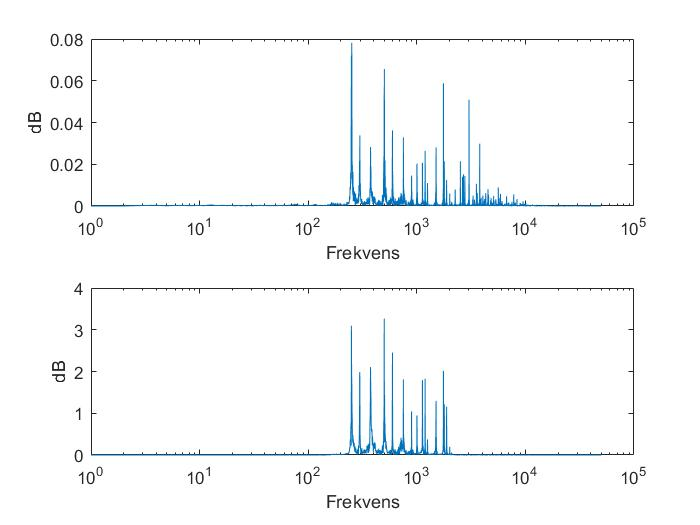
\includegraphics[width=150mm]{figures/Sonata1.jpg}
	\caption{Audio Equalizer på Sonata piano med vægtning 0,0,100,1,1}
	\label{fig:Sonata1}
\end{figure}



\subsection{Vægtning på (10,100,0,1,1)}

\begin{figure}[H]
	\centering
	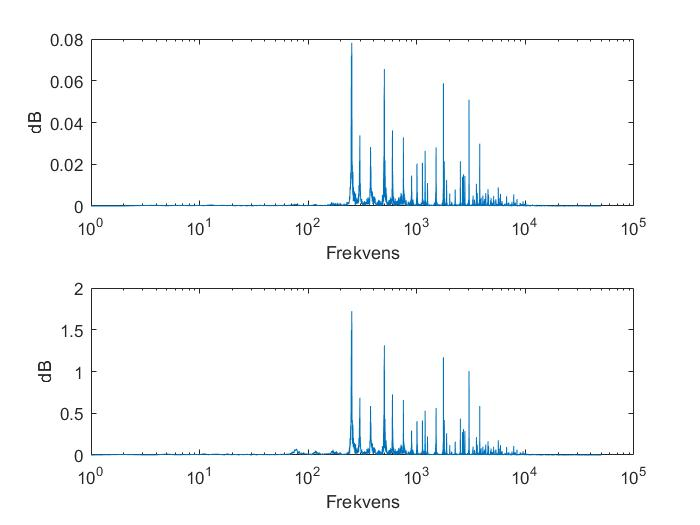
\includegraphics[width=150mm]{figures/Sonata2.jpg}
	\caption{Audio Equalizer på Sonata piano med vægtning 10,100,0,1,1}
	\label{fig:Sonata2}
\end{figure}


\subsection{Vægtning på (100,0,0,10,100)}

\begin{figure}[H]
	\centering
	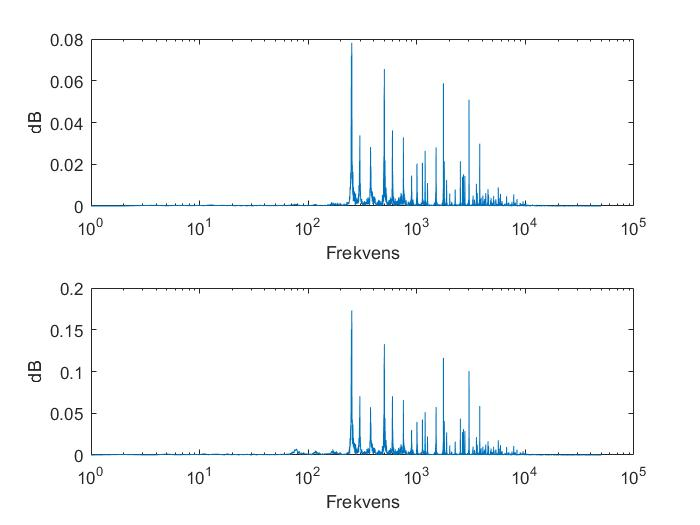
\includegraphics[width=150mm]{figures/Sonata3.jpg}
	\caption{Audio Equalizer på Sonata piano med vægtning 100,0,0,10,100}
	\label{fig:Sonata3}
\end{figure}


\subsection{Vægtning på (1,10,0.1,0.1,1)}

\begin{figure}[H]
	\centering
	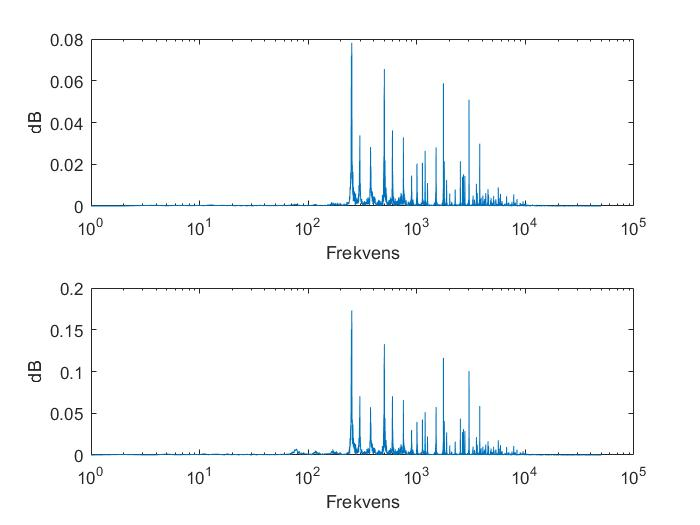
\includegraphics[width=150mm]{figures/Sonata4.jpg}
	\caption{Audio Equalizer på Sonata piano med vægtning 1,10,0.1,0.1,1}
	\label{fig:Sonata4}
\end{figure}
